\subsection{研究目标}\label{ch2target}

由于测试方法的可解释性不足,测试人员无法根据测试结果对深度学习模型进行诊断和调试,用户也很难根据测试结果对模型产生足够的
信任。针对这一问题,传统基于人工(专家)分析的方法可以对深度学习模型的测试结果进行解释,但是,基于人工分析的测试解释方法
受限于专家知识,并且会产生显著的人工费用和时间开销。面对大量测试数据,单纯的依靠人工分析获得可解释的测试反馈,可行性有
限,而现有的解释性方法与可解释的深度学习测试之间还存在不小的距离。面向深度学习模型测试的可解释性不足这一显著问
题,\textbf{本项目的研究目标是:提出一种自动化的、可解释的深度学习模型测试方法,能够在不同测试场景下建立具有语义逻辑的测
    试覆盖指标,辅助测试人员诊断和调试模型,并对测试集生成和测试逻辑进行准确的解释和说明,从而提高深度学习模型测试的可信
    度。}本项目的研究工作对于深度学习应用的开发人员、测试人员和用户来说具有重要的应用价值,对智能软件(如自动驾驶软件)的测
试研究、可信软件的研究和人工智能的可解释性研究具有重要的意义。

\subsection{研究内容}\label{ch2content}

针对深度学习模型的可解释测试方法研究,如\Cref{fig:ch2:rc}所示,本项目拟展开\textbf{可解释性的测试覆盖指标研究和可解释的
    测试集生成技术研究两方面主要研究内容,每个研究内容又包含了多个关键技术点的研究}。通过这两个核心方面的技术研究,完成自动
化的、可解释的深度学习模型测试方法的设计与实现。以下针对这两个方面的研究内容进行相应的描述和解释。

\begin{figure}[htp]
    \begin{small}
        \begin{center}
            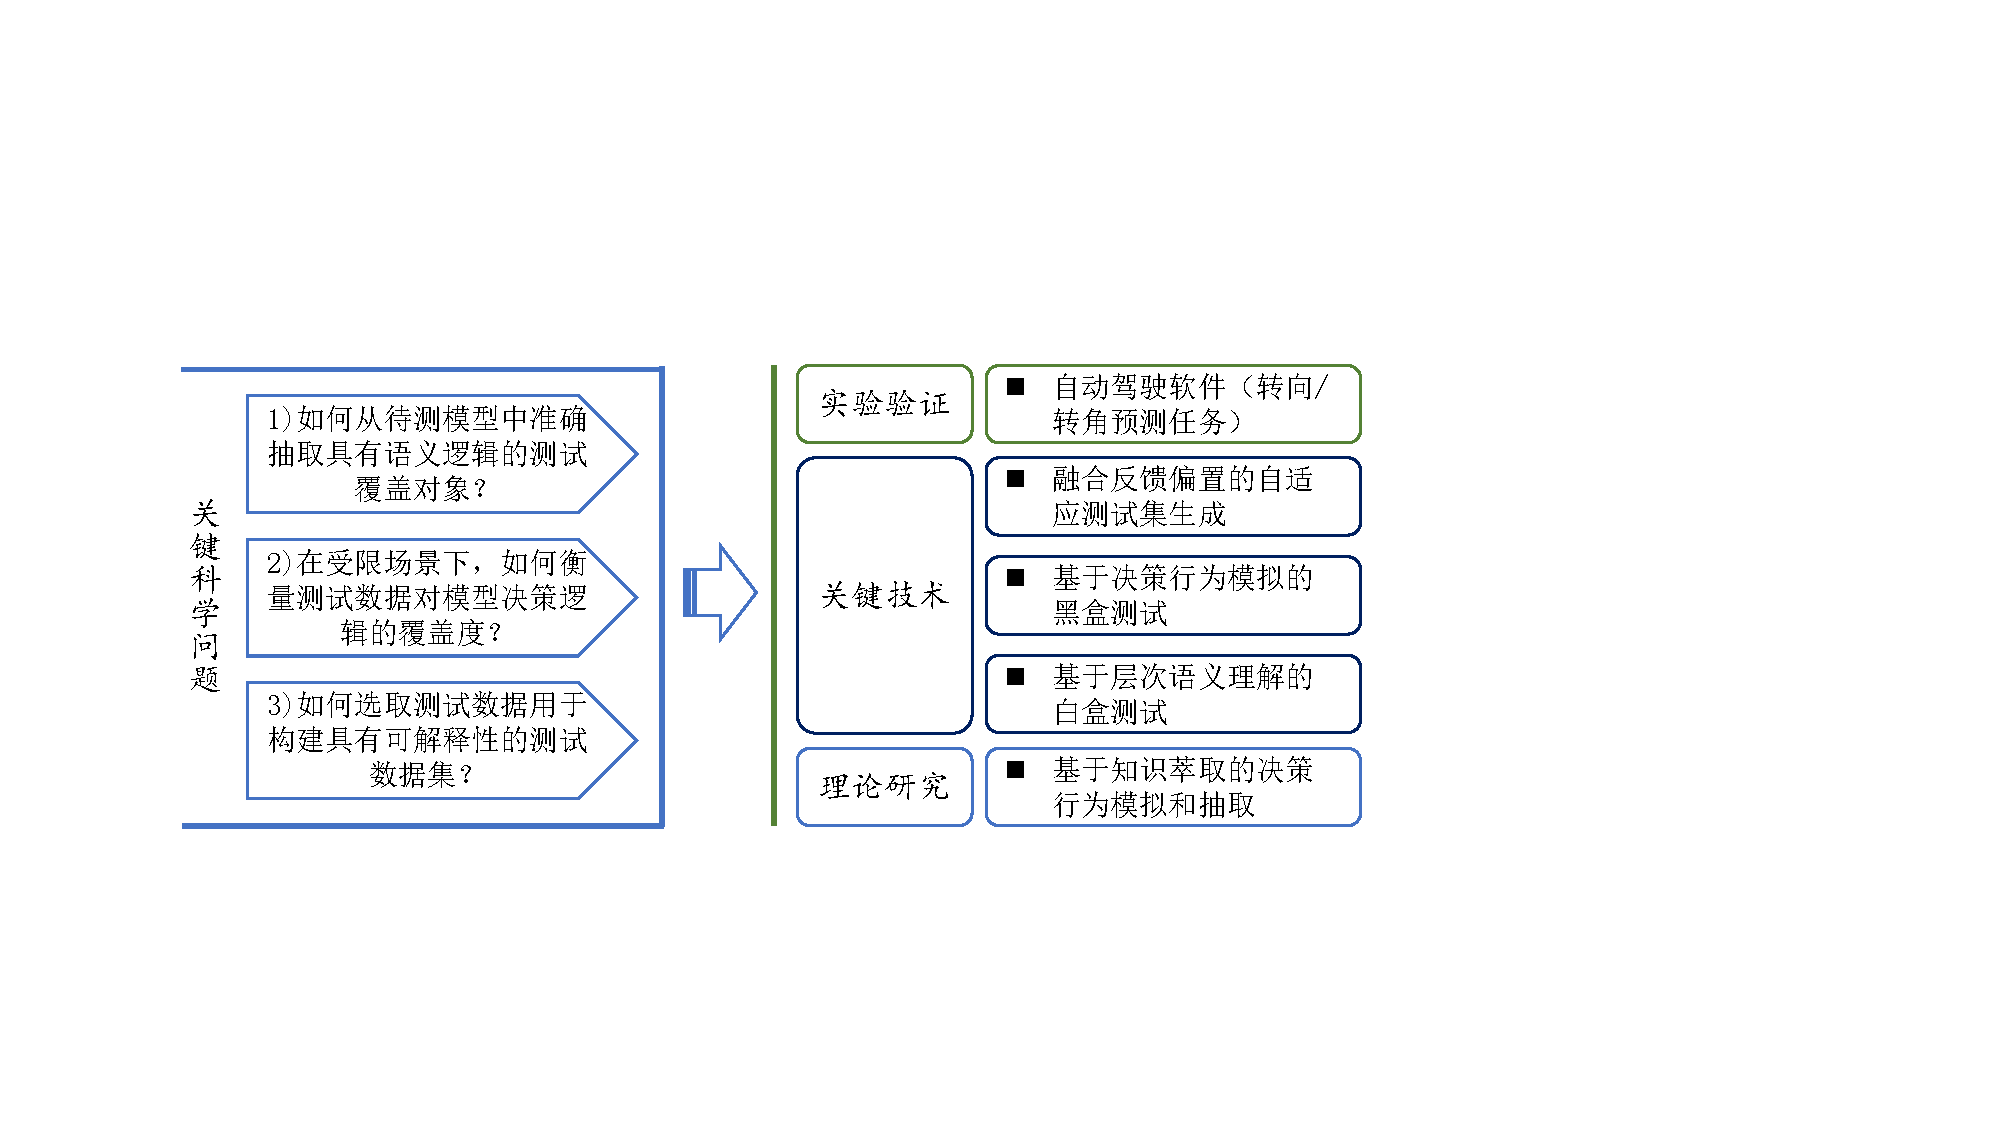
\includegraphics[width=0.95\textwidth]{ch2_RC.pdf}
        \end{center}
        \caption{挑战、科学问题和研究内容关系图}
        \label{fig:ch2:rc}
    \end{small}
\end{figure}

\subsubsection{可解释的测试覆盖指标研究}
根据国内外研究现状,现有的深度学习模型测试方法的可解释性十分有限,相关研究工作还非常缺乏。\textbf{针对深度学习模型测试方
    法的可解释性研究工作,测试覆盖指标的缺乏可解释性是显著的挑战之一,也是难点之一}。测试覆盖指标缺乏可解释性导致:a)以
提高测试覆盖率为目标的深度学习测试方法缺乏明显的测试逻辑;b)测试数据的覆盖特征向量无法体现模型的决策路径和决策依据,
很难通过测试执行情况来检查模型是否在以符合人类认知的形式正常工作;c)测试结果缺乏可解释性,测试人员无法知道测试执行失
效的原因,因此无法根据测试结果来辅助诊断模型缺陷。因此,亟待开展针对深度学习模型的可解释测试覆盖指标研究,并在此基础
上展开以下技术研究工作:\textbf{a)研究针对深度学习模型隐藏层的测试语义抽取技术;b)研究在知识受限场景下的决策逻辑模拟
    技术;c)研究可解释的测试覆盖指标构建方法。}针对测试覆盖指标的可解释性研究作为深度学习模型测试的可解释性研
究的基础,对可解释测试方法的设计与实现中多个关键技术有十分重要的支撑作用。

\subsubsection{可解释的测试集生成技术研究}
由于深度学习模型的输入空间通常存在大量无标注数据,如何从这些数据中选取更有价值的测试数据进行标注和测试,合理平衡测试集的
规模和质量,是测试集生成技术的主要研究内容。根据国内外研究现状,现有的针对深度学习模型的测试集生成方法缺乏容易被测试人员
和用户理解的测试逻辑,测试人员无法解释测试集的充分性和代表性,用户在不了解测试集的情况下很难根据测试覆盖率等指标对模型产
生足够的信任。因此,亟待开展对深度学习模型的可解释测试集生成技术的研究,并在此基础上展开以下技术研究工作:\textbf{a)研究
    测试数据的检测能力分析方法;b)研究大规模无标注数据的代表数据选择技术;c)研究具有可解释性的边界数据选择技术。通过可解释的
    测试覆盖指标和测试集生成方法,实现一种针对深度学习模型的自动化、可解释的测试方法}。


\subsubsection{基于层次语义理解的白盒测试}

除了黑盒测试的场景,白盒测试的需求也非常多,如企业自己开发的深度学习模型,在白盒
测试中,测试者可以访问模型的内部结构$\mathcal M(\bm W, \bm b)$和训练数据集
$\mathcal D_{train}=\{(x^{(i)}, y^{(i)}\})$。目前,针对深度学习模型的白盒测试方
法可扩展性和可解释性较差,无法应用于大规模深度学习模型,如
BERT~\cite{kenton2019bert},MAE~\cite{he2021masked}等,而且测试结果无法给模型训
练提供有效反馈,辅助模型优化。因此,\textbf{本项目提出针对白盒深度学习模型的层次
    语义理解方法,并利用各层的决策语义训练一个副本模型中,保证副本模型的决策路径与原
    白盒模型一致;然后围绕副本模型进行决策路径覆盖度测试,决策路径具有较强的可解释
    性,可引导测试数据生成和模型优化。}

\begin{figure}[htp]
    \begin{small}
        \begin{center}
            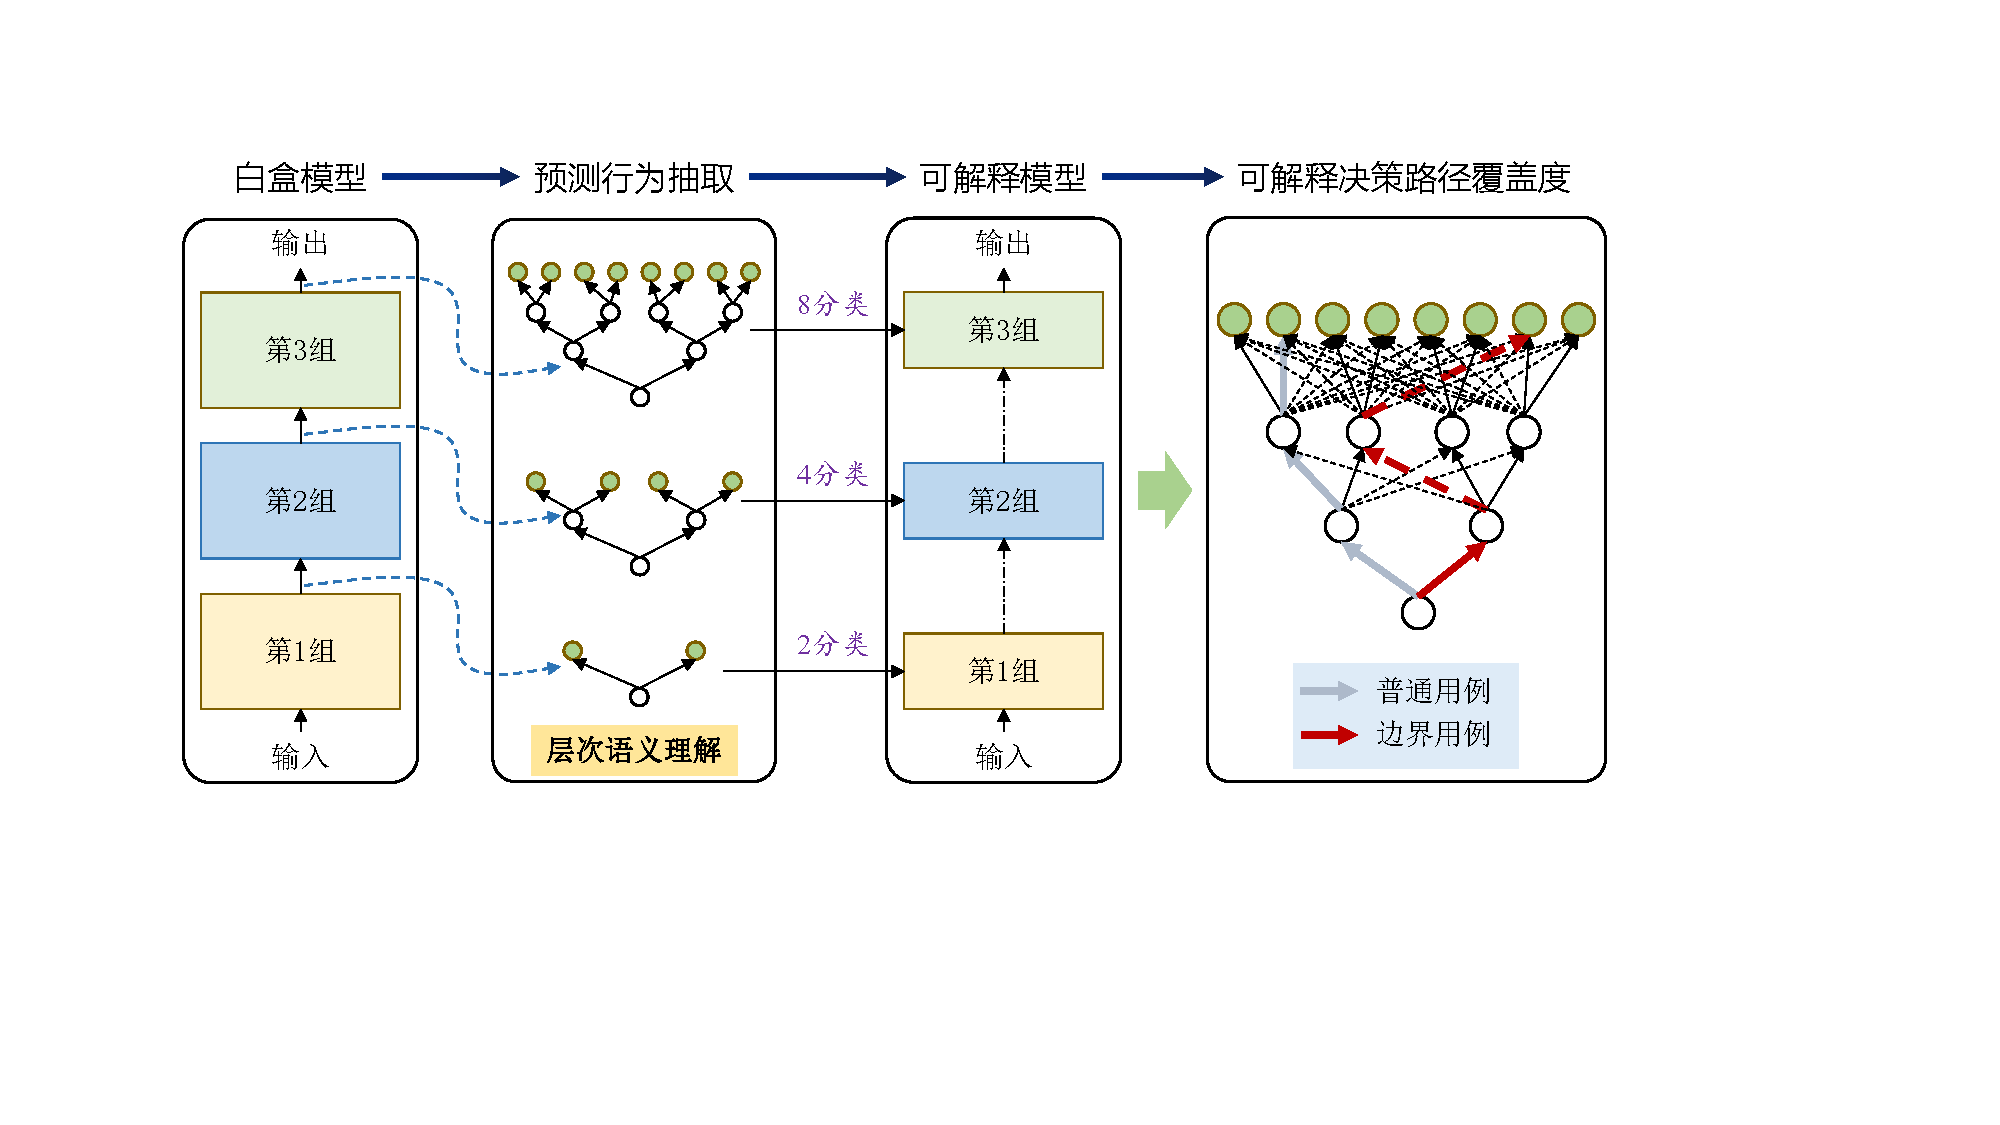
\includegraphics[width=0.9\textwidth]{ch2_WBtest.pdf}
        \end{center}
        \caption{基于层次语义理解的白盒测试研究内容}
        \label{fig:ch2:WBtest}
    \end{small}
\end{figure}

本项目基于层次语义理解的白盒测试研究内容如\cref{fig:ch2:WBtest}所示,在白盒测试
的场景下,本项目首先研究如何从深度学习模型中抽取出各层(layer)的决策语义信息,
研究表明,深度学习模型对输入的决策是由粗粒度到细粒度的。\cref{fig:ch2:WBtest}举
例说明了从3组神经网络层的输出抽取各组网络的预测行为,例如:输入一个猫的图片,第1
组神经网络判断该图片是否是动物,接着,第2组神经网络判断该图片是否是猫科动物,最
后,第3组神经网络将该图片分类为猫。\textbf{本项目拟研究如何实现层次语义理解,自
    动地从深度学习模型中抽取出各层的决策语义}。

在层次语义理解的基础上,\textbf{本项目拟融合白盒模型的多层次决策语义训练一个副本
    模型,使该副本模型的决策路径与原白盒模型一致,且具有良好的可解释性}。此外,知识
蒸馏得到的模型通常规模较小,和直接测试原白盒模型相比,测试副本模型可有效提高测试
效率。\textbf{在得到可解释的副本模型后,本项目拟研究并提出针对该可解释模型的决策
    路径覆盖度,用于分析测试样本的多样性和充分性}。

\subsubsection{融合反馈偏置的自适应测试集生成}
深度学习模型的测试依赖于有标签的测试集,以判断模型预测结果是否符合预期,然而,测
试集的标签通常依赖于人工标注,成本较高,而测试集规模较大,难以标注并测试每个输入
数据。因此,{需要合理平衡测试集的规模和质量,在有限标注成本空间内选取根据测试目
标选取测试数据,生成规模可控制的高质量测试集}。\textbf{本项目拟提出一种基于决策
    路径的自适应测试集生成方法,针对大规模无标注测试数据,融合反馈偏置和自适应测试,
    筛选出具有不同检测能力的测试数据,生成规模可控的高效测试集。}

\begin{figure}[htp]
    \begin{small}
        \begin{center}
            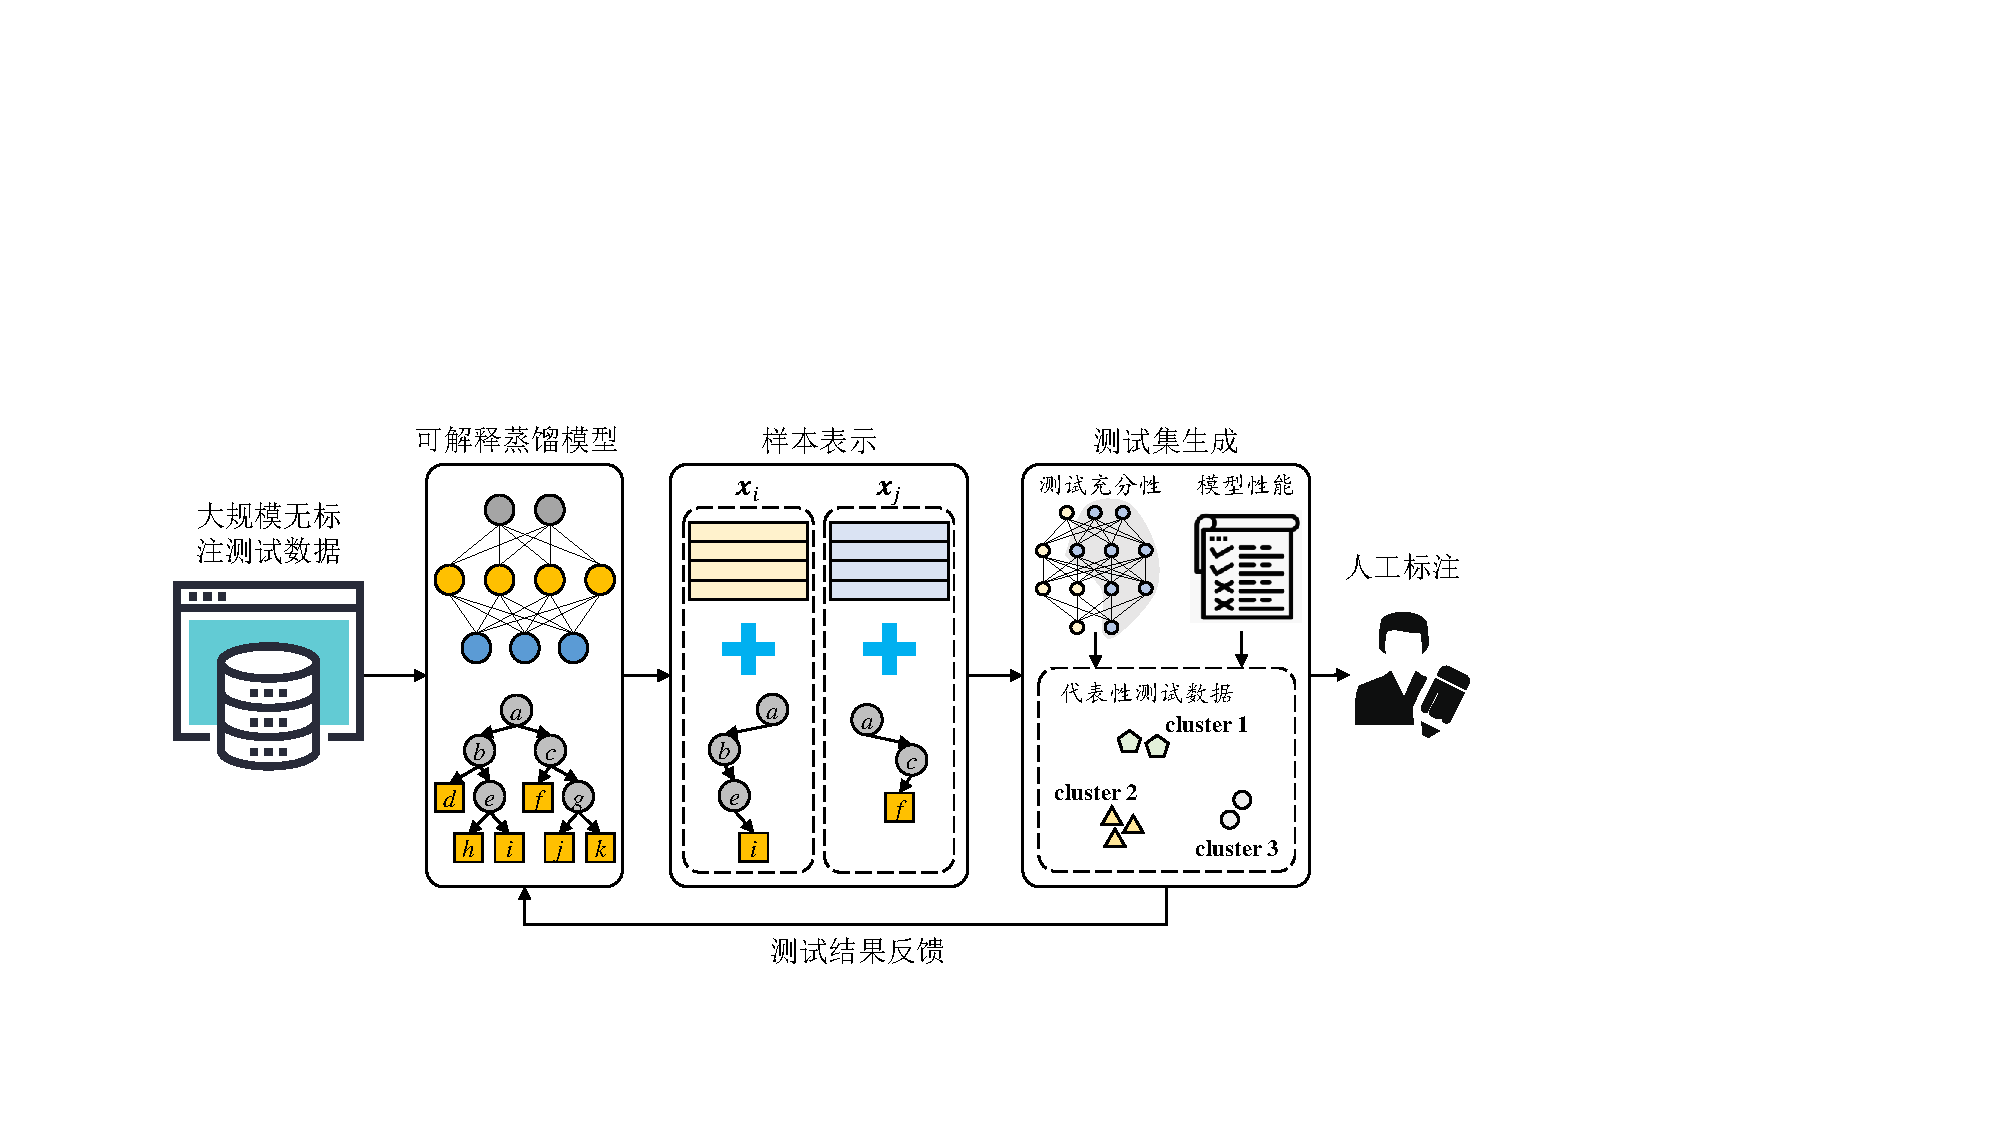
\includegraphics[width=0.95\textwidth]{ch2_TestSelection.pdf}
        \end{center}
        \caption{可解释预测模型研究内容}
        \label{fig:ch2:testselection}
    \end{small}
\end{figure}

如\cref{fig:ch2:testselection}所示,给定大规模无标注测试数据,{本项目选取两类测
试数据构建测试集:\textbf{一类是代表性数据},即能够模拟大规模无标注测试数据分布
的小规模测试子集,以达到高效度量模型性能的目的;\textbf{第二类是边界数据},融合
自适应测试和反馈偏置,找到可能导致模型错误行为的边界测试数据,以达到充分性测试的
目的}。针对第一个测试目标,本项目拟研究样例测试数据选取,结合决策路径和样本表
示,构建可解释的代表性测试集生成方法。针对第二个测试目标,本项目拟融合自适应测试
和反馈偏置,对已选取的测试数据进行标注并测试,并根据测试结果的反馈偏置,持续性筛
选未标注测试数据中的离群点和可能导致模型错误行为的边界数据。


%1.代表性数据筛选,能够用小规模测试数据模拟大规模无标注数据的决策路径分布,准确评估模型性能

%2.边界数据选取,对模型进行充分性测试,找到导致模型错误行为的测试数据标注



\subsection{拟解决的关键科学问题}

基于上述研究目标和研究内容,本项目拟在以下几个关键理论和技术问题上有所突破:

\subsubsection{在黑盒场景下,仅根据模型输入输出,模拟构建黑盒模型的决策路径}

在黑盒测试中,测试者无法了解待测模型的内部结构和训练数据集,仅能得到测试输入输
出,因此无法知晓模型对输入样本是如何决策判断的。现有测试覆盖指标主要基于神经网络
结构的覆盖,仅有黑盒测试研究局限于与模型无关的测试数据多样性的评估,尚未建立模型
有关的黑盒测试方法,无法提供针对特定模型的测试逻辑。因此,在黑盒测试中,如何通过
输入输出模拟模型的决策路径,建立基于决策路径的测试覆盖度指标,以实现可解释黑盒测
试是本项目拟解决的一个关键科学问题。


\subsubsection{在白盒场景下,分层抽象模型内在决策路径,建立基于决策路径的测试覆盖指标}

在白盒测试中,测试者可以得到模型的内部结构和训练数据集,但是深度学习模型的可解释
性差,难以知晓模型对于特定样本是如何决策判断的。另一方面,现有深度学习测试的研究
主要围绕神经元取值和覆盖度进行分析,不仅计算复杂度高,难以应用于大模型,而且缺乏
语义可解释性,相应的测试报告无法给模型开发人员提供有效指导。因此,在白盒测试中,
如何分层抽象深度学习模型内在的决策路径,以实现基于决策路径的可解释测试是本项目拟
解决的另一个关键科学问题。

\subsubsection{在决策路径覆盖引导下,融合反馈偏置筛选规模可控的测试数据评估模型性能}

深度学习模型测试依赖于数据标注,实际应用中,需要合理平衡测试集的规模和质量,在有
限标注成本空间内选取对样本空间最具代表性的测试数据。在本项目黑盒和白盒决策路径覆
盖测试的基础上,已选择的测试数据执行结果可为后续测试数据选择提供模型正确性反馈和
路径覆盖反馈,指导后续测试数据筛选方式,因此,如何对这种反馈偏置进行形式化建模,
将其用于代表性测试用例的持续筛选中,并适应不同的测试目标,也是本项目拟解决的关键
科学问题问题之一。